\section{Formation Background}\label{sec:problem}
Consider a swarm $\mathcal{N}$ of $n$ robots labeled $i\in\left\{1,...,n\right\}$. The swarm is modeled as a directed sensing graph $\mathcal{G}=\left(\mathcal{V},\mathcal{E}\right)$, where vertex set $\mathcal{V} = \left\{1,..., n\right\}$ represents the robots, and edge set $\mathcal{E}\subseteq\mathcal{V}\times \mathcal{V}$ includes robot pairs $\left(i, j\right)\in\mathcal{E}$ for which robot $i$ can sense robot $j$. Denote $\mathcal{N}_i=\left\{j\in\mathcal{V}|\left(i,j\right)\in\mathcal{E}\right\}\subset\mathcal{V}$ as the set of $n_i$ neighbors of a robot $i$ in $\mathcal{G}$.

In this work, the dynamics of the robots are represented in discrete time. Denote $\mathbf{p}_i(k),\mathbf{v}_i(k),\mathbf{u}_i(k)\in\mathbb{R}^3$ respectively be the position, velocity and control input of robot $i$ at time $t(k) = k\tau$, where $\tau$ is the sampling period. The robots in the swarm are homogeneous with a body radius $r$. Each robot is equipped with an inertial measurement unit (IMU) to determine its position and orientation, a range sensor to scan the environment, and a wireless ad-hoc network module to carry out peer-to-peer communication with other robots. In this work, the communication delay between each pair of robots is negligible~\cite{AlonsoMora2018,9527169}. The range sensor provides a $360^\circ$ field of view with the scanning area $S_s$ of radius $r_s$, as shown in Figure~\ref{fig:model}. Its point data obtained at time $t(k)$ is represented by set $\mathcal{M}_i(k)=\left\{\mathbf{m}\right\}$.
\begin{figure}
    \centering
    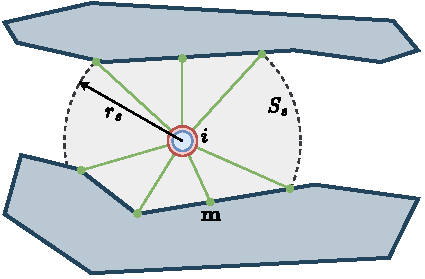
\includegraphics[width=0.48\textwidth]{paper3/images/model.pdf}
    \caption{Illustration of a robot with its range sensor having the scanning area $S_s$ (dashed gray circle) of radius $r_s$ and set $\mathcal{M}_i=\{\mathbf{m}\}$ (green) of the acquired point data.}
    \label{fig:model}
\end{figure}

According to~\cite{Soria2021}, the robot in the swarm can be represented as a discrete linear system as follows:
\begin{equation}
    \mathbf{x}_i(k+1)=\mathbf{A}_i\mathbf{x}_i(k) + \mathbf{B}_i\mathbf{u}_i(k),
\end{equation}
where $\mathbf{A}_i$ and $\mathbf{B}_i$ are system matrices, $\mathbf{u}_i$ is input acceleration, and $\mathbf{x}_i=\left[\mathbf{p}_i;\mathbf{v}_i\right]\in\mathbb{R}^6$ is a state vector including position and velocity. The velocities and accelerations are bounded, i.e., $\mathbf{v}_\text{min}\leq \mathbf{v}_i(k)\leq \mathbf{v}_\text{max}$ and $\mathbf{u}_\text{min}\leq \mathbf{u}_i(k)\leq \mathbf{u}_\text{max}$.